\documentclass[11pt]{article}
\usepackage{graphicx}
\usepackage{hyperref}
\usepackage{natbib}
\usepackage{indentfirst}
\setlength{\textwidth}{6.5in}
\setlength{\headheight}{0in}
\setlength{\textheight}{8.0in}
\setlength{\hoffset}{0in}
\setlength{\voffset}{0in}
\setlength{\oddsidemargin}{0in}
\setlength{\evensidemargin}{0in}

\title{Krishna's First Problem Set}
  
\author{Krishna N. Dindial}


\begin{document}

\maketitle


\section{Introductory Paragraph}
\label{sec:intro}

I went to the NYU Gallatin School of individualized Study for my undergraduate degree and graduated in 2021. My background with programming includes the NYU physics curriculum and comp-sci 101, which was basically an introduction to object oriented programming in Java. I also took a music/tech class called digital electronics in which I used an worked with Arduino software and hardware. For the past year and a half, I have been working as a research associate at Javad Shabani's lab. We probe superconducting microwave circuits with a VNA at microwave frequencies, and I plot and fit the data in a jupyter notebook.
\par On the first day of class, professor Blanton mentioned that there is an ongoing struggle to chose between doing computational projects the "quick and dirty way" and doing the thing the "correct way." That really resonated with me because I often feel forced into doing things the quick and dirty way because I have deadlines and I feel that I don't have the background or training to do things the proper way. In this course I want to learn the how to organize my computational projects and execute them the "proper way" so that when I have to make this choice, its for a good reason, not just because I could only figure out the "quick and dirty way". I often struggle and get frustrated when it comes to coding projects. It is the type of lab work that I feel I am the worst at. In this class I hope to learn the good habits that will minimize the time I feel like I am banging my head against the wall.
\par After grad school I will most likely go to Industry. I have a few friends/colleagues who graduated from Shabani's lab working in industry at IBM or QCI, and it seems appealing to me to be able to work on similar research to do research on superconducting microwave circuits, but have the resources of a private company.

\section{Github}

Here is my github repo: https://github.com/kdindial/phys-ga2000

\begin{figure}[b!]
\centering
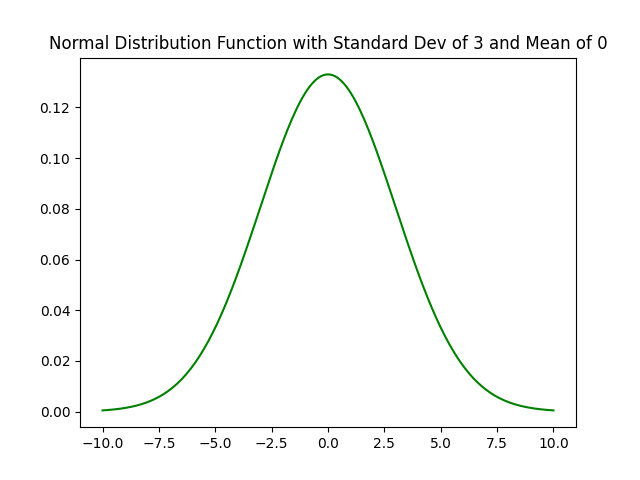
\includegraphics[width=0.95\textwidth]{gaussian.png}
\caption{ \label{fig:example} This is the gaussian plot I made for my first problem set.}
\end{figure}
\end{document}

 
 
